\subsection{Pruning}\label{subsec:pruning}

Some of the semantics from \cref{subsec:semantics} can lead to TAs of an explosive size.
An optional pruning step is performed on the TA, in order to remove transitions, states,
and clocks, that do not affect the transition system.
This leads to better readability, and performance (see \cref{sub:benchmark_uppaal} and \cref{sub:benchmark_treat}).
\vspace{.5\baselineskip plus 2pt}

Throughout this section the TA seen on \cref{fig:prune0} will be used as an example of how the prunings work.
The TA is equivalent to the following TRE, although a few states have been pruned already to make it fit on the page.
$$C(A[5;10]\&(BA|A)[1;3])$$

% Generated by: TimedRegex, Version = 1.0.0.0
% Date 5/14/2024 6:44:16 PM
\usetikzlibrary {automata,positioning}
\scalebox{0.9}{
    % "C(A[5;10]&(BA|A)[1;3])"
    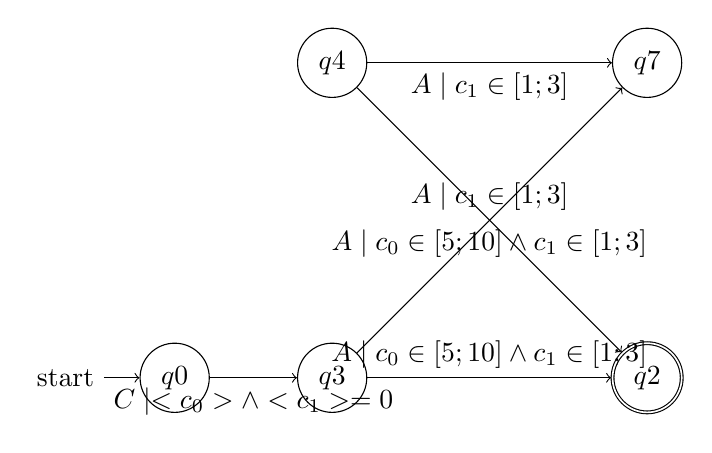
\begin{tikzpicture}[auto]
        \node[state, initial] at (0, 0)(q0){$q0$};
        \node[state] at (2, 0)(q3){$q3$};
        \node[state] at (2, 4)(q4){$q4$};
        \node[state] at (6, 4)(q7){$q7$};
        \node[state, accepting] at (6, 0)(q2){$q2$};
        
        \path[->]
            (q4)edge node[below]{$A\mid c_1\in[1;3]$}(q7)
            (q3)edge node[above]{$A\mid c_1\in[1;3]$}(q7)
            (q4)edge node[below]{$A\mid c_0\in[5;10]\wedge c_1\in[1;3]$}(q2)
            (q3)edge node[above]{$A\mid c_0\in[5;10]\wedge c_1\in[1;3]$}(q2)
            (q0)edge node[below]{$C\mid <c_0>\wedge<c_1>=0$}(q3)
            ;
    \end{tikzpicture}
}

\captionof{figure}{Lightly pruned automaton, to be used as an example.}
\label{fig:prune0}

\subsubsection{Clock Reduction}\label[subsubsection]{clockReduction}
The amount of clocks in the TA can be reduced after generating the TA.
The "Reducing the number of clock variables of timed automata" paper by Daws et al. describes these methods \cite{Daws1996}.
Therefore, we won't go into detail about it in this paper.
We will use $\clockreduction\automaton$ as a function reducing the clocks of TA $\automaton$.

In the TA in \cref{fig:prune0}, both clock $c_0$ and $c_1$ can be combined into one clock since they are reset at the same time.
The result of this operation can be seen in \cref{fig:prune1}.

% Generated by: TimedRegex, Version = 1.0.0.0
% Date 5/14/2024 6:44:16 PM
\usetikzlibrary {automata,positioning}
% "C(A[5;10]&(BA|A)[1;3])"
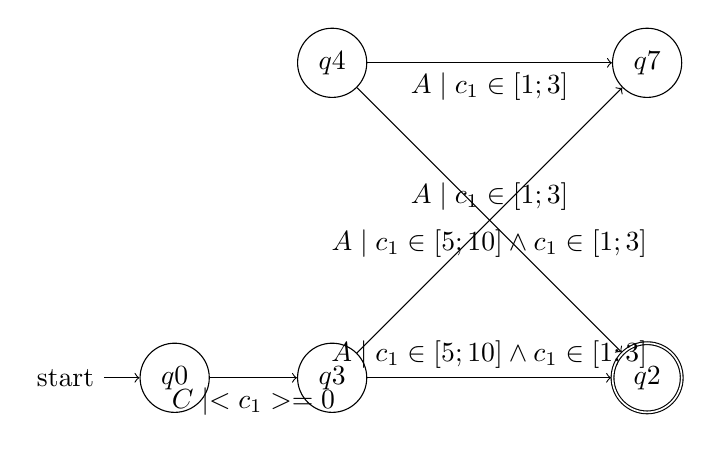
\begin{tikzpicture}[auto]
    \node[state, initial] at (0, 0)(q0){$q0$};
    \node[state] at (2, 0)(q3){$q3$};
    \node[state] at (2, 4)(q4){$q4$};
    \node[state] at (6, 4)(q7){$q7$};
    \node[state, accepting] at (6, 0)(q2){$q2$};
    
    \path[->]
        (q4)edge node[below]{$A\mid c_1\in[1;3]$}(q7)
        (q3)edge node[above]{$A\mid c_1\in[1;3]$}(q7)
        (q4)edge node[below]{$A\mid c_1\in[5;10]\wedge c_1\in[1;3]$}(q2)
        (q3)edge node[above]{$A\mid c_1\in[5;10]\wedge c_1\in[1;3]$}(q2)
        (q0)edge node[below]{$C\mid <c_1>=0$}(q3)
        ;
\end{tikzpicture}
 


\subsubsection{Dead Transition Pruning}\label[subsubsection]{deadTransitionPruning}
Transitions that have unsatisfiable constraints, are considered "dead" transitions, and can be removed without changing the language of the TA.
Since these transitions could never be taken by any transition system, removing them does not change the language.
Dead transition pruning is formally defined in \cref{definition:deadEdgePruning}.

\vspace{0.75em}
Pruning dead edges means pruning all edges that can never be taken because they are overconstrained.

We do this by first taking the intersection of all edges with multiple ranges.
If this intersection has no possible values we know the edge cannot possibly be taken.
Since it cannot be taken we can remove it.

Mathematically this can be described as a function ($\mathbb{E}$) taking in an automaton and returning a new automaton with the dead edges being pruned.

\sembox{
    $\deadedge(A)=\automaton[][Q][C][\Delta'][\Sigma][s][F]$
 
    $\Delta'=\{\transition\in\Delta\mid\phi\neq\emptyset\wedge\emptyset\neq\cap_{i=1}^n\phi_i\}$

}
\vspace{0.75em}

In the TA on \cref{fig:prune1}, we can see that after merging the two clocks, the clock intervals on $q3\rightarrow q2$ and $q4\rightarrow q2$ can be simplified to false:
$$c_1\in[5;10]\wedge c_1\in[1;3]=false$$
A clock can not have a value bigger than 5 and smaller than 3 at the same time.
Since the transition can now no longer be taken, it can easily be removed.
The result of this operation can be seen in \cref{fig:prune2}.

% Generated by: TimedRegex, Version = 1.0.0.0
% Date 5/14/2024 6:44:16 PM
\usetikzlibrary {automata,positioning}
\scalebox{0.9}{
    % "C(A[5;10]&(BA|A)[1;3])"
    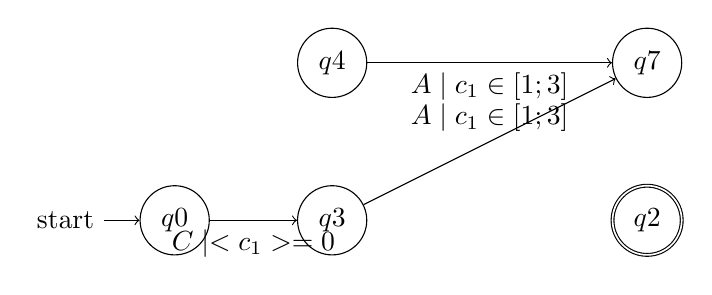
\begin{tikzpicture}[auto]
        \node[state, initial] at (0, 0)(q0){$q0$};
        \node[state] at (2, 0)(q3){$q3$};
        \node[state] at (2, 2)(q4){$q4$};
        \node[state] at (6, 2)(q7){$q7$};
        \node[state, accepting] at (6, 0)(q2){$q2$};
        
        \path[->]
            (q4)edge node[below]{$A\mid c_1\in[1;3]$}(q7)
            (q3)edge node[above]{$A\mid c_1\in[1;3]$}(q7)
            (q0)edge node[below]{$C\mid <c_1>=0$}(q3)
            ;
    \end{tikzpicture}
}

\captionof{figure}{Dead transitions $q4\rightarrow q2$ and $q3\rightarrow q2$ have been removed.}
\label{fig:prune2}


\subsubsection{Unreachable State Pruning}\label[subsubsection]{unreachableStatePruning}
States that are not the destination of any transition or the initial state, are considered "unreachable" states, and can be removed without changing the language of the TA.
Since these states can never be reached, they are not part of the transition system for any words recognized by the TA, hence it does not change the language to remove them.
Unreachable state pruning is formally defined in \cref{definition:unreachableStatePruning}.

\vspace{0.75em}
Unreachable states are very similar to dead states.
Except we check for any edges that end at a given state.
If a state is not reachable it is removed.
Repeat until no such states exist.

\sembox{
    $\unreachable(A_1)=\left\{\begin{array}{ll}
        A_1 & if \forall q_1\in Q_1:q_1'\notin F_1\wedge\transition[_1]\in\Delta_1 \\
        \unreachable(\automaton[][Q][C_1][\Delta][\Sigma_1][s_1][F_1]) & otherwise \\
    \end{array}\right.
    $

    $Q=\{q_1'\in Q_1\mid q_1\notin F_1\wedge\transition[_1]\in\Delta_1\}$

    $\Delta=\{\transition[_1]\in\Delta_1\mid q_1'\in Q\}$
}
\vspace{0.75em}

In the TA in \cref{fig:prune2}, $q4$ and $q2$ can be removed since they are neither the destination of any transition, nor the initial state.
This means there is no way to enter $q4$ or $q2$, and they can be removed.
The result of this operation can be seen in \cref{fig:prune3}.

% Generated by: TimedRegex, Version = 1.0.0.0
% Date 5/14/2024 6:44:16 PM
\usetikzlibrary {automata,positioning}
\scalebox{0.9}{
    % "C(A[5;10]&(BA|A)[1;3])"
    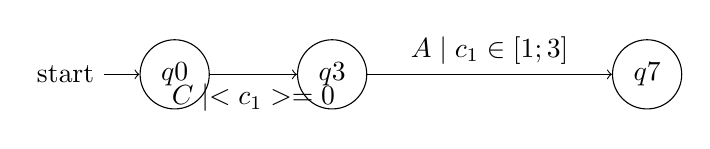
\begin{tikzpicture}[auto]
        \node[state, initial] at (0, 0)(q0){$q0$};
        \node[state] at (2, 0)(q3){$q3$};
        \node[state] at (6, 0)(q7){$q7$};
        
        \path[->]
            (q3)edge node[above]{$A\mid c_1\in[1;3]$}(q7)
            (q0)edge node[below]{$C\mid <c_1>=0$}(q3)
            ;
    \end{tikzpicture}
}

\captionof{figure}{Unreachable states $q4$ and $q2$ have been removed.}
\label{fig:prune3}


\subsubsection{Dead State Pruning}\label[subsubsection]{deadStatePruning}
States that are not final states, or the source of any transition,
are considered "dead" states, and can be removed without changing the language of the TA.
Since these states can not reach final states, they are not part of the transition system for any words recognized by the TA, hence it does not change the language to remove them.
Dead state pruning is formally defined in \cref{definition:deadStatePruning}.

\vspace{0.75em}
Dead states are all the states that have no way of reaching the final state.
These states are pruned by removing all states that have no edges away from them unless they are final states, this is repeated untill no states satisfy this property.

\sembox{
    $\deadstate(A_1)=\left\{\begin{array}{ll}
        A_1 & if \forall q_1\in Q_1:q_1\notin F_1 \transition[_1]\in\Delta_1 \\
        \deadstate(\automaton[][Q][C_1][\Delta][\Sigma_1][s_1][F_1]) & otherwise \\
    \end{array}\right.
    $

    $Q=\{q_1\in Q_1|q_1\notin F_1\wedge\transition[_1]\in\Delta_1\}$

    $\Delta=\{\transition[_1]\in\Delta_1|q_1\in Q\}$
}
\vspace{0.75em}

In the TA in \cref{fig:prune3}, $q7$ can be removed since it is neither the source of any transition, nor a final state.
This means there is no way to reach a final state from $q7$, and it can be removed.
The result of this operation can be seen in \cref{fig:prune4}.

% Generated by: TimedRegex, Version = 1.0.0.0
% Date 5/14/2024 6:44:16 PM
\usetikzlibrary {automata,positioning}
% "C(A[5;10]&(BA|A)[1;3])"
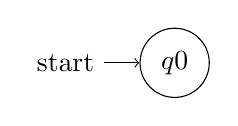
\begin{tikzpicture}[auto]
    \node[state, initial] at (0, 0)(q0){$q0$};
    
    \path[->]
        ;
\end{tikzpicture}
 


\subsubsection{Dead Clock Pruning}\label[subsubsection]{deadClockPruning}
Clocks that are never used in ranges to constrain any transitions, are considered "dead", and can be removed without changing the language of the TA.
Since these clocks never constrain any transitions, it does not change the possible ways to reach final states, hence it does not change the language to remove them.
This rule is formally defined in \cref{definition:deadClockPruning}

\vspace{0.75em}
% Any clocks that are not used in any intervals can be removed.
% This means removing them both from the clocks set and from any clock resets.
% This shouldn't have a huge impact, but it will allow us to create a more minimal declaration field in Uppaal.
\begin{definition}\label{definition:deadClockPruning}
    Dead clock pruning:
    \vspace{0.5em}

    \sembox{
        $\deadclock\automaton=\automaton[][Q][C'][\Delta'][\Sigma][s][F]$

        \vspace{0.5em}

        $C'=\{c\mid\exists\transition[]\in\Delta:\exists(c',I) \in\phi:c=c'\}$

        $\Delta'=\{\transition[][q][q'][\phi][p\cap C']\mid\transition\in\Delta\}$
    }
\end{definition}
\vspace{0.75em}

In the TA in \cref{fig:prune4}, we can see that clock $c_0$ is not being used.
This clock is reset on the transition $q0\rightarrow q3$.
This means we can remove the clock, since it does not affect the ability to take any transitions.
The result of this operation can be seen in \cref{fig:prune5}.

% Generated by: TimedRegex, Version = 1.0.0.0
% Date 5/14/2024 6:44:16 PM
\usetikzlibrary {automata,positioning}
% "C(A[5;10]&(BA|A)[1;3])"
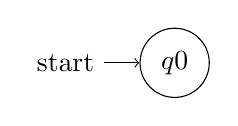
\begin{tikzpicture}[auto]
    \node[state, initial] at (0, 0)(q0){$q0$};
    
    \path[->]
        ;
\end{tikzpicture}
 


\subsubsection{Recursive pruning}
All the prunings described in this section need to happen recursively to get rid of everything.
The recursion stops when no changes have been made to the TA.
This recursion is formally defined in \cref{definition:recursivePruning}

\vspace{0.75em}
\begin{definition}\label{definition:recursivePruning}
    Recursive pruning:
    
    \sembox{
        $\pruning(A)=\left\{\begin{array}{ll}
            A & \text{if }A=A' \\
        \pruning(A') & otherwise \\
        \end{array}\right.
        $

        $A' = \clockreduction\circ\deadedge\circ\deadstate\circ\unreachable\circ\deadclock(A)$
    }
\end{definition}
\vspace{0.75em}

In the TA in \cref{fig:prune5}, there are still things left to be pruned.
The state $q3$ is a dead state and can therefore be removed.
The recursion will take care of that and turn the TA into the one in \cref{fig:prune6}.

% Generated by: TimedRegex, Version = 1.0.0.0
% Date 5/14/2024 6:44:16 PM
\usetikzlibrary {automata,positioning}
\scalebox{0.9}{
    % "C(A[5;10]&(BA|A)[1;3])"
    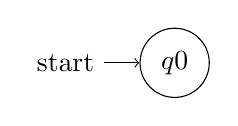
\begin{tikzpicture}[auto]
        \node[state, initial] at (0, 0)(q0){$q0$};
    \end{tikzpicture}
}

\captionof{figure}{Final pruned automaton.}
\label{fig:prune6}
